%%%%%%%%%%%%%%%%%%%%%%% file typeinst.tex %%%%%%%%%%%%%%%%%%%%%%%%%
%5
% This is the LaTeX source for the instructions to authors using
% the LaTeX document class 'llncs.cls' for contributions to
% the Lecture Notes in Computer Sciences series.
% http://www.springer.com/lncs       Springer Heidelberg 2006/05/04
%
% It may be used as a template for your own input - copy it
% to a new file with a new name and use it as the basis
% for your article.
%
% NB: the document class 'llncs' has its own and detailed documentation, see
% ftp://ftp.springer.de/data/pubftp/pub/tex/latex/llncs/latex2e/llncsdoc.pdf
%
%%%%%%%%%%%%%%%%%%%%%%%%%%%%%%%%%%%%%%%%%%%%%%%%%%%%%%%%%%%%%%%%%%%


\documentclass[runningheads,a4paper]{llncs}

\usepackage[latin1]{inputenc}
\usepackage{graphicx,color,url}
\usepackage[dvips]{epsfig}
\usepackage{verbatim}
\usepackage{tikz}
\usetikzlibrary{shapes,arrows}
\usetikzlibrary{calc,patterns,snakes,decorations.pathmorphing,decorations.markings}
\usetikzlibrary{positioning}

\providecommand{\tabularnewline}{\\}





\usepackage{amssymb}
\setcounter{tocdepth}{3}
\usepackage{graphicx}

\usepackage{url}
\urldef{\mailsa}\path|salemohammed@gmail.com|
\urldef{\mailsb}\path|amorag@geneura.ugr.es, jjmerelo@gmail.com|
%\urldef{\mailsc}\path| fergunet@gmail.com|
\newcommand{\keywords}[1]{\par\addvspace\baselineskip
	\noindent\keywordname\enspace\ignorespaces#1}

\begin{document}
	
	\mainmatter  % start of an individual contribution
	
	% first the title is needed
	\title{Evolving a TORCS Fuzzy driver using Genetic Algorithms}
	
	
	%\titlerunning{Driving in TORCS using modular fuzzy controllers}
	
	
	
	
%	\author{Mohammed Salem* \inst{1} \and Antonio Miguel Mora \inst{2}\and Juan Julian Merelo \inst{2} \and Pablo Garc\'ia-S\'anchez \inst{3}}
% Antonio - The submission is blind. ;)
	
	
	%\authorrunning{M. Salem et al}
	% (feature abused for this document to repeat the title also on left hand pages)
	
	% the affiliations are given next; don't give your e-mail address
	% unless you accept that it will be published
%	\institute{University of Mascara, Algeria\\
%		\mailsa\\
%		Department of Architecture and Computer Technology
%		University of Granada, Spain\\
%		\mailsb\\
%		Universiy of C\'adiz, Spain
%		\\
%		\mailsc\\
%	}
% Antonio - The submission is blind. ;)

	%
	% NB: a more complex sample for affiliations and the mapping to the
	% corresponding authors can be found in the file "llncs.dem"
	% (search for the string "\mainmatter" where a contribution starts).
	% "llncs.dem" accompanies the document class "llncs.cls".
	%
	
%	\toctitle{Driving in TORCS using modular fuzzy controllers}
%	\tocauthor{}
	\maketitle
	\begin{abstract}
		
		This work presents an evolutionary approach to optimise the parameters of Fuzzy-based controller for an autonomous driver for the open simulated car racing game (TORCS). The aim is to improve a modular fuzzy agent designed to determine the optimal target speed and steering angle during the race.
These kinds of controllers have a big drawback, which is their membership function parameters are tuned by a trial-error process.
Thus, a real-coded Genetic Algorithm 
% Antonio - TODO: Extend the description of the algorithm.
has been applied to find the best values for these parameters, which let us to design a robust driver for this racing simulator.
The evolved drivers were compared and  evaluated in practise and realistic races, yielding very good results mainly in tracks that have many turning points, which are, in turn, the most difficult for any autonomous agent.
% Antonio - TODO: describe the experiments performed and say something else about the results.
	%%%
	\keywords{Videogames, Fuzzy Controller, TORCS, Steering control, Optimization, Genetic Algorithms}
	\end{abstract}
% Antonio - I have rewritten the abstract. It was very similar to the one of last year. ;)

%%%%%%%%%%%%%%%%%%%%%%%%%%%%%%%   INTRODUCTION   %%%%%%%%%%%%%%%%%%%%%%%%%%%%%%%
	%
	\section{Introduction}
	\label{sec:intro}

% Antonio: TODO - write the Introduction.
Autonomous driving is a very interesting research topic recently supported by many vehicle manufacturers. The final aim is to create real self-driving cars that can move in everyday roads or, for instance, in a desert or hostile environment. This objective is complemented with the reduction of fuel consumption and the maximisation of its efficient use, along with the car safety and the driver comfort.

The Open Racing Car Simulator (TORCS) \cite{WebTORCS} is a realistic racing simulator with a sophisticated engine used for many standalone racing competition challenges every year. This fact, combined with the large gaming community and the ability to compare controllers have made TORCS the most used simulator in the field of autonomous driving [***,***,***].
% Antonio - add some references about research in TORCS (from those commented in the State of the art)

One of the most efficient controllers so far applied in this environment are fuzzy-based ones, as they simulate in part the human reasoning when driving. In this line, the authors presented previously an approach in which two specialised fuzzy controllers were combined to decide the car's steering angle and desired speed in every single point during a race \cite{evo17_blind}. 
% Antonio - citation to our previous work without authors nor title since this is a blind revision process
% Antonio - Mohammed, was these factors computed every small amount of time or just in some parts of the track, such as in every curve?
The obtained results were promising, but the performance of the autonomous driver showed some flaws in difficult tracks - where `external' factors affected the asphalt - and against the most competitive rivals.
We argue here that the major disadvantage of this approach is that the parameters of the controllers' fuzzy membership functions were defined following a trial/error process in the absence of experts to do so.

Thus, in this work we consider the selection of the best values for these parameters as an optimisation problem, so we have applied an evolutionary algorithm to obtain them. Concretely, we propose to apply a real-coded Genetic Algorithm (GA) \cite{GAs_Goldberg89} 
% Antonio - Look for a citation to a real-coded GA?
with this purpose. The considered approach requires - in addition to a good codification of solutions and selection of operators - the choice of an adequate cost function (fitness), due to the uncertainty and noisiness of the problem itself, so two different implementations have been studied.

% Antonio - TODO: Comment about the obtained results

%%%%%%%%%%%%%%%%%%%%%%%%%%%%%%  STATE OF THE ART  %%%%%%%%%%%%%%%%%%%%%%%%%%%%%%
	\section{State of the Art}
	\label{sec:soa}

% Antonio: TODO - write the State of the art.


%%%%%%%%%%%%%%%%%%%%%%%%%%%%%%  TORCS  %%%%%%%%%%%%%%%%%%%%%%%%%%%%%%

\section{ TORCS Description: }
	\label{sec:torcs}
% Antonio - TODO: Maybe reduce it (if we go beyond 16 pages). ;)
The Open Racing Car Simulator (TORCS) is an open source, modern, multi-player, modular and portable racing simulator that allows users to race against computer-controlled opponents. TORCS allows the user to control one of the robots through an input device such as keyboard, mouse or joystick \cite{manualTORCS}.

Its high degree of modularity and portability make it ideal for artificial research. Indeed, a number of competitions and research-based papers have already appeared that make use of the TORCS  engine\cite{WebTORCS}. Because of these features, the simulator has become popular and interesting as it provides real-time driving simulation\cite{manualTORCS}.  The game allows different types of races from the practical single session to the championship \cite{manualTORCS}.

%%%%%%%%%%%%%%%%%%%%%%	
	\begin{table}[ht!]
		{\scriptsize
			{\centering
				\begin{tabular}{|p{2cm}|p{3cm}|p{3 cm}|p{3 cm}|}
					\hline
					{\textbf{Sensor} }&
					{\textbf{Name} }&
					{\textbf{Range} (unit)} &  
					{\textbf{Data type}}\\ 
					\hline
					1 & angle & [-$\pi$,+$\pi$ ] & Double\\ 
					\hline
					2 & curLapTime & [0,+$\infty$] (s)	& Double\\ 
					\hline 
					3 & damage & [0,+$\infty$)(point)& Double\\ 
					\hline 
					4 & distFromStart & [0,+$\infty$) (m)& Double \\ 
					\hline 
					5 & distRaced &[0,+$\infty$) (m)& Double\\
					\hline 
					
					6 & focus & [0,200] (m)& Double\\
					\hline 
					
					7 & fuel & [0,+$\infty$) (l)& Double\\
					
					\hline
					8 & gear & \{-1,0,1,.. 6\}g& Integer \\
					
					\hline
					9 & lastLapTime &[0,+1] (s) & Double \\
					
					\hline
					10 & opponents &[0,200] (m)& Double \\
					
					\hline
					10 & racePos & \{1,2,...,N\} & Double \\
					\hline
					11 & rpm    & [0,+$\infty$) (rpm)   & Double \\
					\hline  
					13 & speedX & (-$\infty$,+$\infty$) (km/h) & Double\\
					\hline  
					14 & speedY &(-$\infty$,+$\infty$) (km/h)  & Double\\
					\hline 
					15 & speedZ & (-$\infty$,+$\infty$) (km/h) & Double \\
					
					\hline
					16 & track &  [0,200 ] & Double\\ 
					\hline
					17 & trackPos & (-$\infty$,+$\infty$) & Double\\
					
					\hline
					
					18 & wheelSpinVel  & [0,+$\infty$) (rad/s) & Double\\
					
					\hline
					19 & z &  (-$\infty$,+$\infty$) (m) & Double\\
					
					\hline
					
				\end{tabular}
			}
		}
		\caption{Description of available sensors in TORCS \cite{Torcs3}.}
		\label{t1}
	\end{table}
	
	Every TORCS driver bot is controlled by means of a set of actuators: the steering wheel `Steer', the accelerator `accel', the brake pedal and the gearbox. In addition, a meta-action is available to request a restart of the race to the server. Table \ref{tab2} details the available actions/actuators and their representation.
	
	\begin{table}[ht!]
		{\scriptsize
			{\centering
				\begin{tabular}{|p{3cm}|p{3 cm}|p{3 cm}|}
					\hline
					
					{\textbf{Action} }&
					{\textbf{Range} (unit)} &  
					{\textbf{Data type}}\\ 
					\hline
					Acceleration & [0,+1] & Double\\ 
					\hline
					Brake & [0,+1]	& Double\\
					\hline
					Gear & -1..0..+6	& Double\\
					\hline
					Steer & [-1,+1]	& Double\\
					\hline
					Clutch & [-1,+1]	& Double\\
					\hline
				\end{tabular}
			}
		}
		\caption{TORCS Actuators \cite{torcs2012}.}
		\label{tab2}
	\end{table}
	
	Hence, a controller is a program, which run inside TORCS, that automatically drives a car. It gets as input information about the current state of the car and its situation on the track. These collected data are used to compute actions to do in the next simulation tick; like steer, gear changes, acceleration or brake and clutch. A client may request a restart of the race by sending a special action on the server: Restart or shutdown \cite{manualTORCS}.
	
	
	%%%%%%%%%%%%%%%%%%%%%%%%%%%  FUZZY CONTROLLER  %%%%%%%%%%%%%%%%%%%%%%%%%%%%
	%
	\section{Fuzzy Controller}
	\label{sec:fuzzy_controller}
	
The proposed controller has the same modular architecture as the simple driver, and has some common functions of this approach. 
However, the target speed and steering angle are computed by means of two modular and specialised fuzzy controllers, which consider five position sensors.

In the following sections, each sub-controller is described.

%-----------------------------------------------

\subsection{Fuzzy target speed sub-controller}

The first proposed fuzzy sub-controller aims to estimate the optimal target speed of the car, both in straight parts and curves of the track, taking into account two criteria: moving as faster as possible and secure the car. This estimation is based on fuzzy rules, so two general cases are considered, following the simple driver approach:

\begin{itemize}
	\item If the car is in a straight line, the target speed will take a maximum value (\textit{maxSpeed} km/h).
	\item If it is close to a curve, the controller will decrease the current speed to a value included in the interval \textit{[minSpeed; maxSpeed]} km/h.
\end{itemize}

Thus, in case the car is out of the track or near a curve, the brake system is activated, and ABS (Anti-Block System) and TCL (Traction Control Limit) will be loaded to avoid the car skidding. The obtained target speed will be used for computing the value of acceleration, following - as the simple driver do - the expression:

\begin{equation}	
Gas(speed-Target_{speed})=-1+\frac{2}{1+e^{speed-Target_{speed}}}	
\end{equation}

\textit{Gas} function refers to acceleration, \textit{speed} is the current speed of the car.

This fuzzy controller has three input values and one output: the target speed .
The presented controller is a Mamdani-based fuzzy system \cite{iancu2012} with trapezoidal Membership Functions (MF) for input variables, because it avoids sudden changes in input values. It considers three values among the 19 track sensors:

\begin{itemize}
	\item Front = Track[9]: the front distance between the car and the border of the track (angle 0�).
	\item M5 = max (Track[8], Track[10]): the max distance to the track limits in an angle of +5� and -5� with respect to Front.
	\item M10 = max (Track[7], Track[11]): the max distance to the border in an angle of +10� and -10�.
\end{itemize}


Each input variable is represented by three membership functions: Low, Medium and High. The description of fuzzy inputs and output are represented in Table \ref{tab:flouevar}.

\begin{table}
	\caption{Fuzzy variables description.}
	\label{tab:flouevar}
	\begin{tabular}{ |p{1.5cm}|p{2cm}|p{2cm}|p{2 cm}|p{1 cm}|p{1.5 cm}|p{1.5 cm}|}
		\hline
		{ \color{red} Variable }&
		{ \color{red} Range }&
		{ \color{red} Name}&  
		{ \color{red} MF } &
		{ \color{red} Low } &
		{ \color{red} Medium }&
		{ \color{red} High } 
		
		\\
		\hline
		\hline
		Input & [0-100] m & Front & trapezoidal & [0-50] & [20-80] & [60-100]
		\\
		\hline
		Input & [0-100] m & M5 & trapezoidal &[0-40] & [10-70] & [50-100] 
		\\
		\hline
		Input & [0-100] m  & M10 & trapezoidal & [0-30] & [20-60] & [50-100]
		\\
		\hline 
		Output & [0-200] m/s & TargetSpeed & singleton & / & / & /
		\\
		\hline 
	\end{tabular} 
\end{table}

The base of rules has been composed modelling the behaviour of a human expert driver, refining them also. Thus, this set is designed so that if the frontal distance is maximal, then the target speed should be the maximum. Its value should be lower when the frontal distance is shorter. 
The fuzzy rules are listed below:

\begin{itemize}
	\item IF Front is High THEN TargetSpeed is TS1
	\item IF Front is Medium THEN TargetSpeed is TS2
	\item IF Front is Low and M5 is High THEN TargetSpeed is TS3
	\item IF Front is Low and M5 is Medium THEN TargetSpeed is TS4
	\item IF Front is Low and M5 is Low and M10 is High THEN TargetSpeed is TS5
	\item IF Front is Low and M5 is Low and M10 is Medium THEN TargetSpeed is TS6
	\item IF Front is Low and M5 is Low and M10 is Low THEN TargetSpeed is TS7\\
	
	In addition, a crisp rule is added to rule base to obtain a maximum value of the target speed when the three input variables are as big as possible: 
	\item IF Front = MAXDISTSPEED or M5 = MAXDISTSPEED or M10 = MAXDISTSPEED THEN TargetSpeed = MAXSPEED		
\end{itemize}

MAXDISTSPEED is the a longest possible value for the track sensors, and MAXSPEED, which is related to the car's properties, is the maximal car speed. For example in the case of car-trb1 model, MAXSPEED=300.

The output value is encoded by seven singletons TS1 to TS7, being respectively: 280, 240, 220, 180, 120, 60 and 30.

%-----------------------------------------------

\subsection{Fuzzy steering control sub-controller}	

In addition to the speed sub-controller, another fuzzy approach has been applied to control the steering, estimating and determining the target position of the car. 

The architecture of this sub-controller is similar to the one shown in Figure \ref{fig:AD}, but with the steering as output. 
% Antonio - This figure is not in this paper. ;)
The set of sensors considered are the same as in the speed case, described in Table \ref{tab:flouevar}.

Then, if the car is in a straight line, it will set as target position half width of the race track (central position of the lane).	Whereas, if the car is near a right curve, it will approach the path leading to the right, with a space between the car and the border of the track to avoid the loss of control. The same approach is considered if the car is near a left curve.

In order to detect the curves, the controller focuses on the sensor values (M10, M5, and Front). So, if the value on Front sensor is the longest, there is a straight road; whereas if the values of M5 and M10 with positive angles (+5 and +10) are the longest, there is right curve; and the other way round.

The base of rules has been defined again modelling the behaviour of a human driver, so, for this controller is:

\begin{itemize}		
	\item IF Front is High THEN steer is S1
	\item IF Front is Medium AND M10 is High THEN  steer is S2
	\item IF Front is Medium AND M10 is Medium AND M5 is Medium THEN steer is S2
	\item IF Front is Medium AND M10 is Medium AND M5 is Low THEN steer is S3
	\item IF Front is Low AND M10 is High THEN steer is S3
	\item IF Front is Low AND M10 is Medium AND M5 is Medium THEN steer is S4
	\item IF Front is Low AND M10 is Medium AND M5 is Low THEN steer is S4
\end{itemize}	

The values for S1 to S4 are respectively: 0, 0.25, 0.5, and 1.
When M10=Track[7] we will take negative values of the steer (steer=-steer).

Once the controllers have been described, they will be tested and compared with the standard one y several races. The obtained results are presented in the following section.

%%%%%%%%%%%%%%%%%%%%%%%%%%%%  OPTIMISING WITH GAS  %%%%%%%%%%%%%%%%%%%%%%%%%%%%
	
\section{Optimizing the fuzzy controllers with GA}

Difficulties 
% Antonio - Which difficulties? Comment them.
in designing fuzzy controllers of TORCS have led us to move towards the use of Genetic Algorithms (GAs) \cite{GAs_Goldberg89} because of their global exploration characteristic in a complex environment, as this problem plots.

The proposed optimization approach aims to find the optimal parameters of the membership functions of the two sub-controllers \cite{evo17_blind} (see Figure \ref{fig:ga}). 
An initial population is drawn randomly and each solution is evaluated through TORCS 
% Antonio - What does 'evolved through TORCS' means? Please, explain it better.
to get the optimal one.
% Antonio - This is the main part of the work, you must explain completely (and very well) the GA procedure. ;)

\begin{figure}[!ht]
	\label{fig:ga}
	\begin{center}
		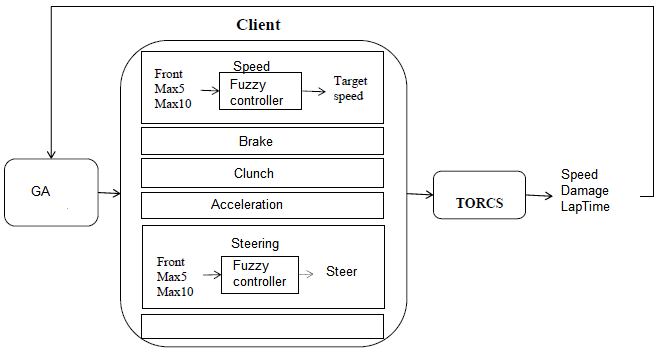
\includegraphics[width=13cm,height=7cm]{fig/mo}
	\end{center}
	\caption{Optimization of fuzzy controller flowchart }
% Antonio - Please, explain deeper the figure. It's not easy to understand
\end{figure}	

%***********************************************
\subsection{Genetic algorithm settings}
%
As previously stated, the designed fuzzy controllers have trapezoidal membership functions given by \ref{eq:trapmf}.
In such a controller, fuzzy rules are applied to linguistic terms. These terms, which qualify a linguistic variable, are defined through membership functions, which, in turn, depend on a set of parameters that `describes' their shape (and operation).
% Antonio - please Mohammed check this text I have added. ;)

The parameters to be optimized are thus defined in two steps: first, the parameters of each membership function must be selected, then all the parameters of the membership functions that constitute the fuzzy partition of the linguistic variable \cite{ThangG08}.
% Antonio - this sentence seems to be incompleted.

A trapezoidal membership function in a finite universe of discourse \textit{[a, b]} can be defined by:

\begin{equation}
\mu_{A}(x)= \left \{
\begin{array}{ll}
\frac{x - x_{1}}{x_{2} - x_{1}},& x_{1} \leq x \leq x_{2}\\
1 , &x_{2} \leq x \leq x_{3}\\
\frac{x_{4} - x}{x_{4} - x_{3}},& x_{3} \leq x \leq x_{4}\\
0        ,& else\\	
\end{array}
\right.
\label{eq:trapmf}
\end{equation}
with:
\begin{equation}
x_{1} \leq x_{2} \leq x_{3} \leq x_{4}
\end{equation}
This MF function is defined by four parameters $x_{1}$, $x_{2}$, $x_{3}$ and $x_{4}$ taking their values in the interval \textit{[a, b]} (See Figure \ref{fig:trapeze}).																			
\begin{figure}[!ht] 
	\begin{center}
		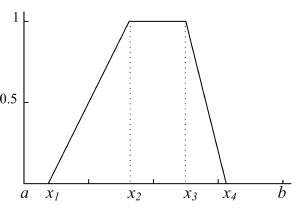
\includegraphics[scale=0.95]{fig/trapese}
		\caption {Trapezoidal MFs}
		\label{fig:trapeze}
	\end{center}
\end{figure}

The input linguistic variables in our problem, \textit{Front, Max5} and \textit{Max10}, are represented by five trapezoidal membership functions (See Table {tab:flouevar}).
More generally, a fuzzy partition with \textit{n} trapezoidal membership functions is defined by \textit{2n} variables (\textit{a =} $ x_{1}$,$x_{2} $,. .., $x_{2n} $ \textit {= b})(Equation \ref{eq:e1}). In this case, the representation is given by the figure \ref{fig:at}
\begin{figure}[!ht] 
	\begin{center}
		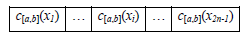
\includegraphics[scale=0.95]{fig/at}
		\caption {Trapezoidal-shaped MFs coding}
		\label{fig:at}
	\end{center}
\end{figure}
with:
\begin{equation}
a = x_{1} \leq x_{2} \leq...\leq x_{2n-1} \leq x_{2n}=b 	
\end{equation}		

\begin{equation} 
\begin{tabular}{l}
$\mu_{A1}(x)=  \left \{
\begin{array}{ll}
1, &x_{1} \leq x \leq x_{2}\\
\frac{x_{3} - x}{x_{3} - x_{2}}, &x_{2} \leq x \leq x_{3}\\
0        , &x > x_{3}\\
\end{array} 
\right.$		\\ 	
$\mu_{Ai}(x)= \left \{
\begin{array}{ll} 
0, &x \leq x_{2i-2}\\
\frac{x - x_{2i-2}}{x_{2i-1} - x_{2i-2}}, &x_{2i-2} \leq x \leq x_{2i-1},n=2,...,i-1\\
1, & x_{2i-1} \leq x \leq x_{2i}\\
\frac{x_{2i+1} - x}{x_{2i+1} - x_{2i}},& x_{2i} \leq x \leq x_{2i+1}\\
0  , &x > x_{2i+1}\\
\end{array}  
\right.	$		\\
$\mu_{An}(x)= \left \{
\begin{array}{ll} 
0, &x \leq x_{2n-2}\\
\frac{x - x_{2n-2}}{x_{2n-1} - x_{2n-2}},& x_{2n-2} \leq x \leq x_{2n-1}\\
1 ,& x > x_{2n-1} 
\end{array} 
\right.$\\
\label{eq:e1}
\end{tabular}
\end{equation}
	
As we have just seen, a linguistic variable is represented by a number of parameters that depend both on the number and type of used membership functions  \cite{ThangG08}. Also the choice of coding to use for these different parameters depends both on the desired precision on the values and on their range of values.

When the number of parameters is reduced and their ranges of variations are well defined, a GA with a binary coding is largely sufficient to find their optimal values. On the other hand, if the number of parameters becomes important, and their variation interval is not well known, the real coding is the most appropriate \cite{elsayed13}. 
Since our work requires some precision and the variation interval of each parameter is not well known, we have considered a real coding implementation.

Usually, the chromosomes of the first population are initialized with random values, however we initialized the membership function parameters randomly but inside their range of variation \cite{3}, in order to start from feasible values. 
% Antonio - another citation is missing.
The figure \ref {fig:cromosome} illustrates the structure of the chromosome.
with  :
% Antonio - Is something missing here? 
\begin{itemize}
	\item []$0 = x_{11} \leq x_{12} \leq x_{13} \leq x_{14} \leq x_{15} \leq x_{16} = 100$
	\item []$0 = x_{21} \leq x_{22} \leq x_{23} \leq x_{24} \leq x_{25} \leq x_{26} = 100$
	\item []$0 = x_{31} \leq x_{32} \leq x_{33} \leq x_{34} \leq x_{35} \leq x_{36} = 100$
\end{itemize}
\begin{figure}[!ht]	
	\begin{center}
		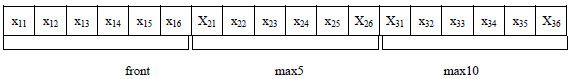
\includegraphics[width=13cm,height=3cm]{fig/cromosome.png}
		\caption{Chromosome description}
		\label{fig:cromosome}	
	\end{center}	
\end{figure}

Tournament based selection has been used to select chromosomes as parents for genetic operators, while simple arithmetic two point crossover is chosen with non uniform mutation.
% Antonio - we should include a reference to any operator. Moreover, it would be great if we can justify why these operators have been selected (instead of others).

%***********************************************
\subsection{Fitness definition}

The fitness function for optimizing the structure of a fuzzy controller is highly dependent on the application in which the controller is involved. It is therefore not possible to give a general formulation of this function able to adapt to all the peculiarities of a problem. However, we can specify some rules to choose the best evaluation function \cite{elsayed13}.

The fuzzy controller should aim to: 
\begin{description}
	\item  Minimize the damage of the car $damage$.
	\item  Minimize the overall race time $RaceTime$.
	\item  Maximize the TopSpeed $MaxSpeed$.		
\end{description}

From this goals, we can derive two possible fitness functions:

\begin{description}
	\item[fitness 1:]  
	\begin{equation} \label{fit1}
	\begin{array}{lllll}
	%f_{cout} =  $min$ & \alpha & $. damage$ + & $min$ &\beta & $. temps$ 
	f_{1} =  Min & damage + &\alpha  Min & RaceTime 
	\end{array}
	\end{equation}
	\item[fitness 2:] 
	\begin{equation} \label{fit2}
	\begin{array}{llllll}
	%f_{cout}= min &\alpha & $. dammage$ + & min &\beta & $. temps$ + & min &\gamma & .\frac{1}{vitesse}
	f_{2}= Min & damage + &\alpha Min & RaceTime+ & Min & \beta \frac{1}{MaxSpeed}
	\end{array}
	\end{equation}	
\end{description}

Being $\alpha$ and $\beta$ two weighting parameters to prioritize the importance of the different objectives.
To evaluate the candidate controllers during the evolutionary process, we will make each of them compete in a 20 laps race 
% Antonio - which kind of race? which track, which conditions, which rivals?
%           This is very important to be mentioned and explained (why have these %           features been selected to correctly evaluate a controller). ;)
and collect the obtained output values ($damage$, $RaceTime$ and $MaxSpeed$) to compute the fitness.


  		
%%%%%%%%%%%%%%%%%%%%%%%%%%%%  SIMULATION RESULTS  %%%%%%%%%%%%%%%%%%%%%%%%%%%%
	
	\section{Simulation Results}
	\label{sec:results}
	
	In this section we present all the experiments that we performed in order to measure the performance of our controller, called \textit{AD (Automatic Driver)}.
	We first, describe the methodology we have used and next, we present the experimental results of the implementation of the fuzzy driver, including opponents and using special criteria in each case.
	
	\subsection{Simulation settings}
	
	TORCS provides several tracks to choose which have been designed in order to test the performance of the controllers on different difficulty circuits and on different types of roads.
	In our case, we chose the E-Track5 circuit
	
	
	Table \ref{Tabtrack} presents the properties and description of selected track.
	
	\begin{table}
		
		\caption{Description of Selected track}
		\label{Tabtrack}
		\begin{tabular}{ |p{2cm}|p{2.2 cm}|}
			\hline
			\textbf{Track name}    & E-Track5	\\
			\hline
			\textbf{Shape}   
			& 
\includegraphics[scale=0.3]{fig/track4.png}			
			\\
			\hline
			\textbf{Track Type}   
			& Oval
			\\
			\hline
			
			\textbf{Length}   
			& 1621.73 m	\\
			\hline
			\textbf{Width}   
			& 20.0 m\\
			\hline
		\end{tabular} 
		
	\end{table}
	
	The aim of this selection is to test the value of AD in a wide set of situations, in order to check its potential as a global controller.
	
	
	% ----------------------------------------------
	
	\subsubsection{Cars settings.}
	
	The car considered is \textit{car1-tbr1} of SCR 1 Server, which is a NASCAR car part of the SCR Server team. It has a weight of 1150 KG, max fuel: 94 KG, length: 4.25m and width: 1.94m, with 300km/h as maximal speed.
	This is a fair car, i.e. not the fastest, but a quite fast. Anyway, the obtained results represents the quality of the controllers and could be extrapolated to any other car.
	
	% ----------------------------------------------
	
	\subsubsection{Controllers settings.}
	
	We have tested the different sub-controller features in a separated way, in order to see which one has the highest influence on the success or failure of
	AD. Thus, we have considered the following bots in the experiments:
	
\begin{enumerate}
	\item AD: Fuzzy controller .
	\item [- AGFC1:] GA-Fuzzy controller with fitness 1 \ref{fit1},
	\item[- AGFC2:] GA-Fuzzy controller with fitness 2 \ref{fit2},
\end{enumerate}	
%

	
	%%%%%%%%%%%%%%%%%%%%%%%%%%%%%%%%%%%%%%%%%%%%%%%%%%%%%%%%%%%%%%%%%%%%

	\begin{table}[!ht]	
		\caption{GA parameters}
		\label{parametre}
		\begin{tabular}{|p{9.6cm}|p{5cm}|}
			\hline \textbf{Population size} & 20 \\
			\hline \textbf{Generations} & 50   \\
			\hline \textbf{Crossover rate$\textit{P}_{\textit{c}}$} &  0.7 \\
			\hline \textbf{Mutation rate $\textit{P}_{\textit{m}}$} &  0.3   \\ 		
			\hline          
		\end{tabular}	
	\end{table}


%%%%%
\subsection{GA-Fuzzy  controller in practice race}
\begin{table}[!ht]
	\caption{Results of the three controllers in a 20 laps practice race}
	\label{resultat20}
	\begin{tabular}{|p{3.5 cm}|p{3.5 cm}|p{3.5 cm}|p{3.5 cm}|}
		\hline
		\multicolumn{4}{|c|}{{\large \textbf{E-Track 5}}}  \\ \hline
		\hline \textbf{20 tours} & \textbf{AD} & \textbf{AGFC1} & \textbf{AGFC2}  \\
		\hline Best Time         & 29:70 & 30:03 & 29:50 \\
		\hline Topspeed          & 209 & 216 & 216\\
		\hline Minspeed          & 168 & 148 & 182 \\
		\hline Time Lastlap      & 29:79 &  30:03 & 29:50\\
		\hline Best lap          & 19/20 &  20/20& 20/20\\
		\hline Damages          & 936 & 0 & 0\\
		%\hline Fuel              & 74:01       &  74:11                 &   \\
		\hline Lap               & 20/20       &  20/20                 & 20/20  \\
		\hline 
		\hline
		\multicolumn{4}{|c|}{{\large \textbf{E-Road}}}  \\ \hline
		\hline \textbf{20 tours} & \textbf{AD} & \textbf{AGFC1} & \textbf{AGFC2}  \\
		\hline Best Time         & 02:31:71    & 02:26:72       & 02:26:54  \\
		\hline Topspeed          & 206         & 205            &  208 \\
		\hline Minspeed          & 30          & 39             & 37  \\
		\hline Time Lastlap      & 03:12:79    &  02:42:26      &  02:33:36 \\
		\hline Best lap          & 02/20       & 02/20          &  02/20 \\
		\hline Damages          &   0         & 0              & 0  \\
		%\hline Fuel                &  & 61:01  &  52:61 \\
		\hline Lap               &   20/20     & 20/20          & 20/20  \\
		\hline 
	\end{tabular}
\end{table}


\subsection{GA-Fuzzy controllers in a real race}
\begin{table}[!ht]
	\caption{Results of AGFC1 in a real race}
	\label{14}
	\begin{tabular}{|p{2.3cm}|p{1.75 cm}|p{1.75 cm}|p{1.75 cm}|p{1.75 cm}|p{1.75 cm}|p{1.75 cm}|}
		\hline \textbf{E-track5} &   \textbf{AGFC1} & \textbf{berwin 10} & \textbf{bt 3} &\textbf{damned 2} & \textbf{inferno 5} & \textbf{contre tita 10}  \\
		\hline \textbf{Ranking} & 3/6&4/6&1/5&5/6&2/6&6/6\\			
		\hline \textbf{Temps total}	& 02:30:74\newline+35:70&02:30:74\newline+1lap&02:30:74&02:30:74\newline+1lap&02:30:74\newline+12:13&02:30:74\newline+1lap\\	
		\hline \textbf{Best Lap}&35:65& 36:39&28:57&36:83&30:53&35:39\\	
		\hline \textbf{Maxspeed}& 196&202&231&192&226&202\\	
		\hline \textbf{Damages}& 0&0&0&603&0&471 \\	
		\hline \textbf{Pit stops} & 0&0&0&0&0&0\\	 
		\hline 
	\end{tabular}
\end{table}
\begin{table}[!ht]
	\caption{Results of AGFC2 in a real race }
	\label{15}
	\begin{tabular}{|p{2.3cm}|p{1.75 cm}|p{1.75 cm}|p{1.75 cm}|p{1.75 cm}|p{1.75 cm}|p{1.75 cm}|}
		\hline \textbf{E-track5} & \textbf{AGFC2}&\textbf{berwin 10} & \textbf{bt 3} &\textbf{damned 2} & \textbf{inferno 5} & \textbf{tita 10}  \\
		\hline \textbf{Ranking} & 2/6&4/6&1/6&6/6&3/6&5/6\\			
		\hline \textbf{Race Time}	& 02:30:83\newline +03:99&  02:30:83\newline+1lap&02:30:83&02:30:83\newline+1lap&02:30:83\newline+08:35&02:30:83\newline+1lap\\	
		\hline \textbf{Best Time}& 29:82 &36:38&28:35&37:04&30:53&36:00\\	
		\hline \textbf{Maxspeed}& 214&202&230&188&226&204\\	
		\hline \textbf{Damages}& 0& 0 & 343&1230&0&668\\	
		\hline \textbf{Pit stops} &0&0&0&0&0&0 \\ 
		\hline 
	\end{tabular}
\end{table}
\begin{table}[!ht]
	\caption{Results of AD in a real race}
	\label{16}
	\begin{tabular}{|p{2.3 cm}|p{1.75 cm}|p{1.75 cm}|p{1.75 cm}|p{1.75 cm}|p{1.75 cm}|p{1.75 cm}|}
		\hline \textbf{E-track5} & \textbf{AD} & \textbf{berwin 10} & \textbf{bt 3} &\textbf{damned 2} & \textbf{inferno 5} & \textbf{tita 10}  \\
		\hline \textbf{Ranking} & 6/6&5/6&1/6&4/6&2/5&3/5\\			
		\hline \textbf{Race Time}	& 02:31:83\newline+5laps&02:31:83\newline+1lap&02:31:83&02:31:83\newline+1lap&02:31:83\newline+21:32&02:31:83\newline+33:43 \\	
		\hline \textbf{Best Time}& 00:00&37:25&28:60&36:28&31:47&35:84\\	
		\hline \textbf{Maxspeed}& 111&202&230&189&225&202\\	
		\hline \textbf{Damages}& 10786&465&5&0&2394&0 \\	
		\hline \textbf{Pit stops} & 0&0&0&0&0&0\\ 
		\hline 
	\end{tabular}
\end{table}



	\section{Conclusions and Future Work} 
\label{sec:conclusions}
\newpage
	\bibliographystyle{splncs03}
	\bibliography{fuzzy_torcs}
	
	
	
	
	
	
\end{document}
